\section{Analysis}\label{sec:results_web_ping}
\subsection{Initial Site Ping Analysis}

The first analyses were conducted directly on the site, live for users to see using the aforementioned D3-powered map view as shown in \cref{fig:siteping_state_view}. Data was aggregated on the server side by state and city so the site could also display ranked states and cities (best and worst). Every new data point caused an update in the analyses -- both for our own uses and to help users understand how their state performs. An example of these rankings is shown in \cref{fig:siteping_rankings}.

\begin{figure}
    \centering
    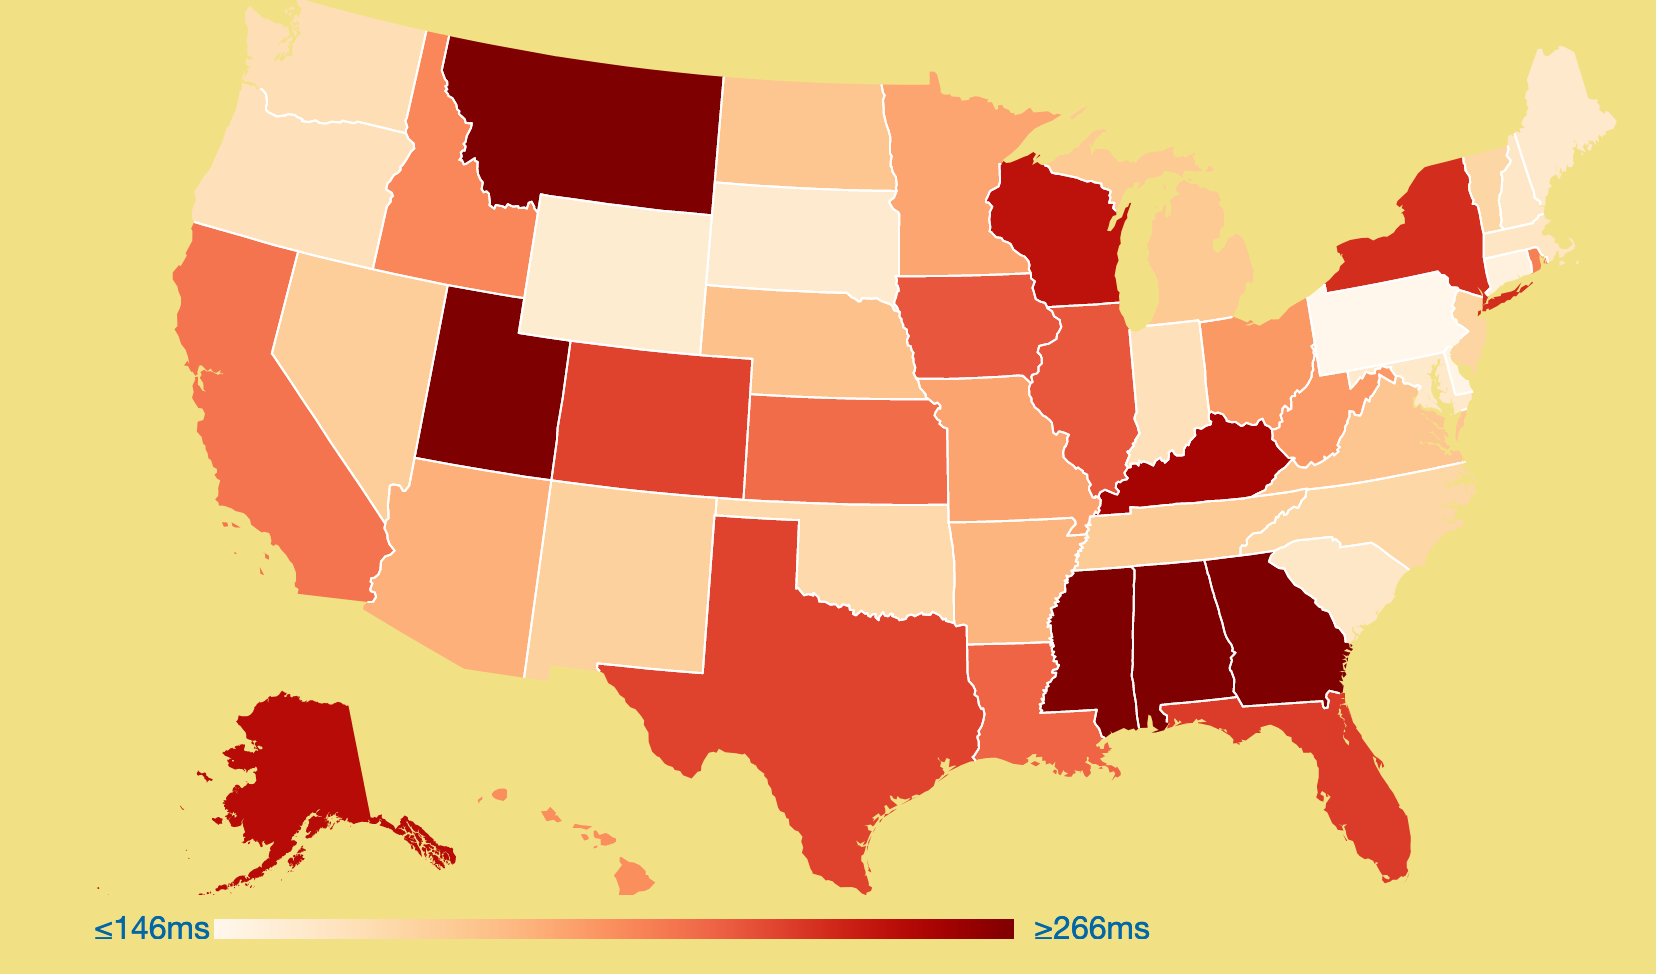
\includegraphics[width=\textwidth]{images/siteping/Siteping_state_map.png}
    \caption{State view chloropleth map}
    \label{fig:siteping_state_view}
\end{figure}

\begin{figure}[h]
    \centering
    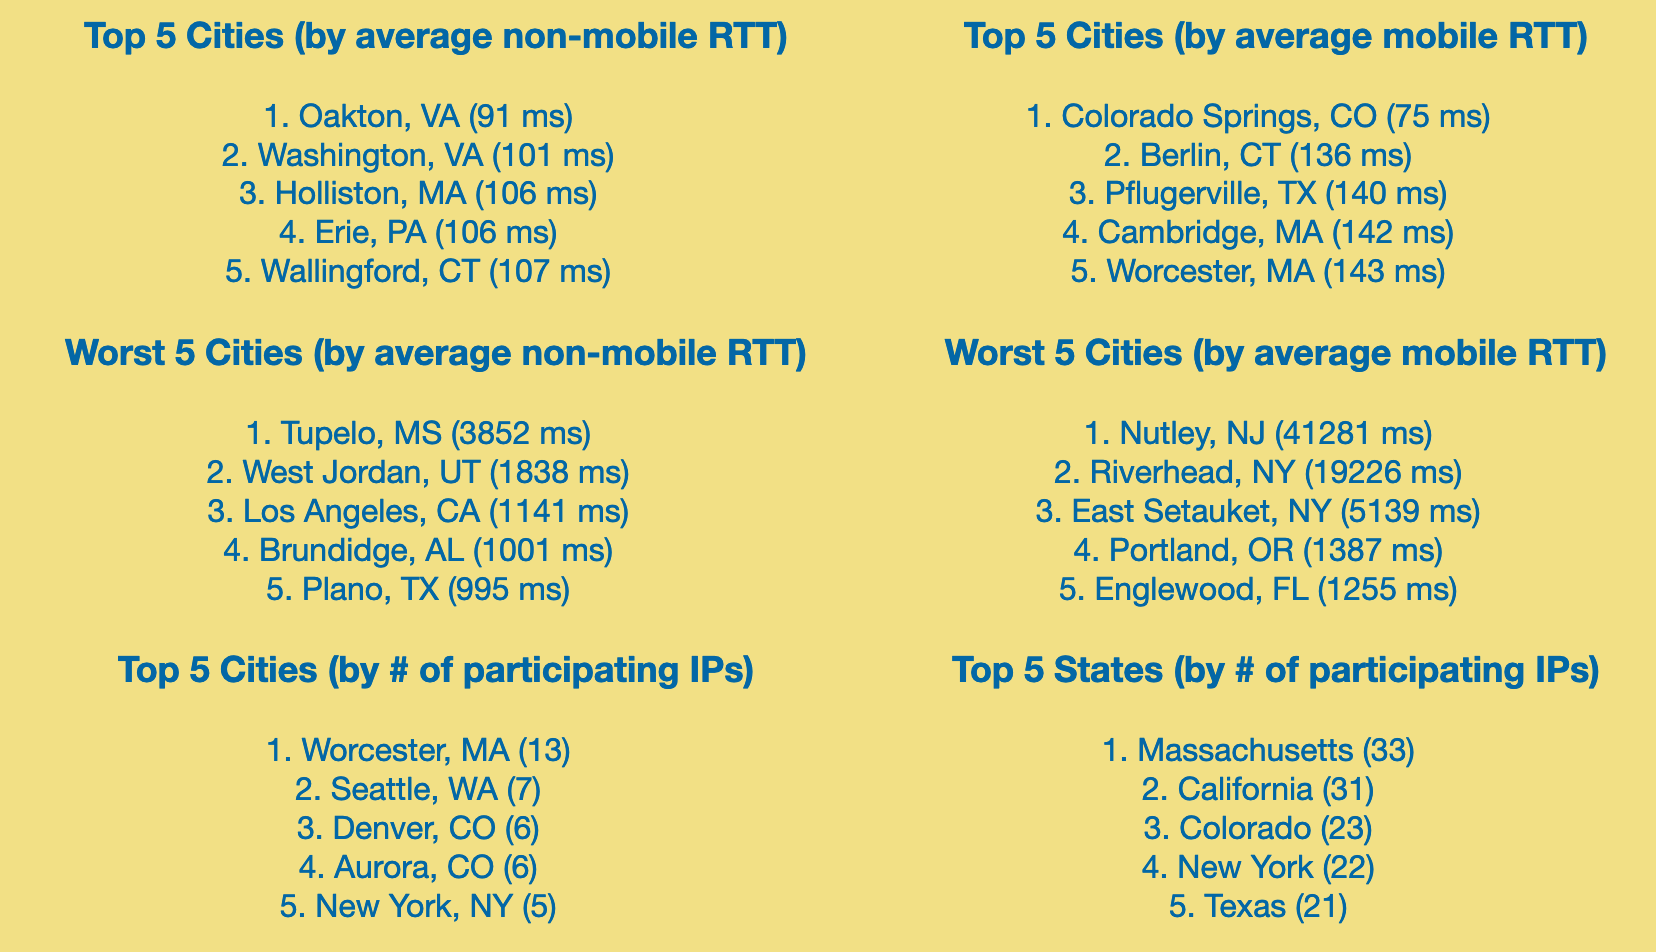
\includegraphics{images/siteping/Sitping_Rankings.png}
    \caption{Site ping live-updating state rankings}
    \label{fig:siteping_rankings}
\end{figure}

\subsection{Data Quality}

\begin{figure}[h]
    \centering
    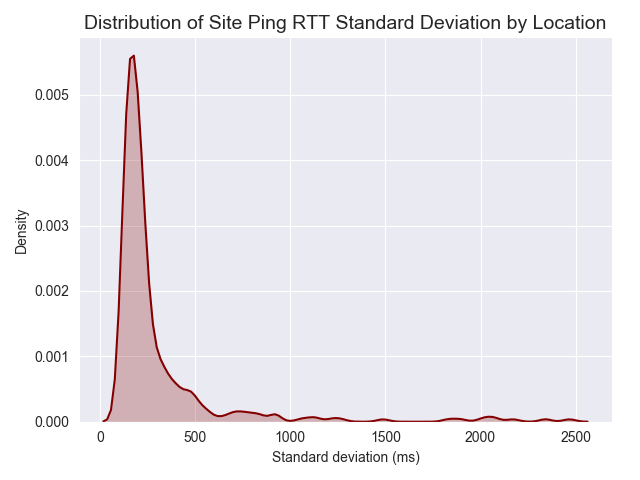
\includegraphics{images/siteping/siteping_rtt_stdev_distribution.png}
    \caption{Distribution of site ping standard deviations by location}
    \label{fig:siteping_stdev_dist}
\end{figure}

The first measure of data quality tried was standard deviation, the per-location distribution of which is shown in  \cref{fig:siteping_stdev_dist}. The chart shows a fairly smooth curve where the overwhelming majority of points have standard deviations of around 150 milliseconds. This is a fairly high standard deviation, most likely caused by the small number of data points for each location.

\begin{figure}[h]
    \centering
    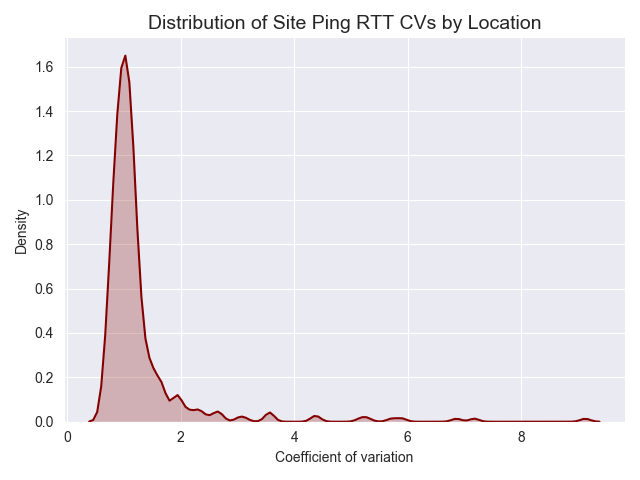
\includegraphics{images/siteping/siteping_rtt_cv_distribution.png}
    \caption{Distribution of Coefficient of Variations pair by location}
    \label{fig:siteping_cv_dist}
\end{figure}

Next, we calculated the \cv for each location, shown in \cref{fig:siteping_cv_dist}. \CVs are dimensionless measures of the ratio between standard deviation and mean, interpreted the same across any data set. Most of the \cvs are around 1, meaning there is significant variance in the data. Again, this is most likely related to the relatively small number of data points that exist for each location.

\subsubsection{Evaluating State Rankings}

\begin{figure}[h]
    \centering
    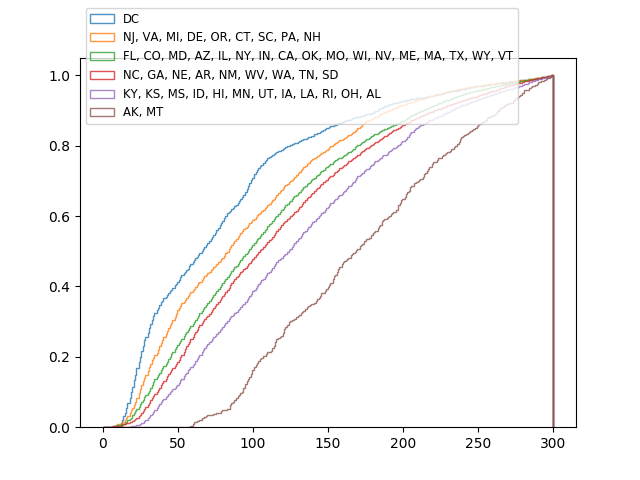
\includegraphics{images/siteping/siteping_clusters_cdf.png}
    \caption{Continuous distribution function of state rankings}
    \label{fig:siteping_cdf}
\end{figure}
\todo{Label these axes?}

To examine whether or not it was statistically allowable to aggregate the data by state, we used the Kruskal-Wallis test, as described in \cref{sec:stats_methods}. \todo{This needs to be fleshed out a LOT}From there we grouped the states into cliques based on weather or not they could be compared with all the other states. \cref{fig:siteping_cdf} shows a \cdf of all of the groupings of states.

\begin{longtable}{lrrr}
\toprule
State &  Value &  n &  Rank \\
\midrule
\endhead
\midrule
\multicolumn{4}{r}{{Continued on next page}} \\
\midrule
\endfoot

\bottomrule
\endlastfoot
DC    &    73.0 &   6845 &     1 \\
DE    &    75.5 &    304 &     2 \\
CT    &    76.0 &   3772 &     3 \\
NH    &    80.0 &   2056 &     4 \\
NJ    &    83.0 &    708 &     5 \\
PA    &    85.0 &   3823 &     6 \\
MI    &    88.0 &   1928 &     7 \\
SC    &    89.0 &   1776 &     8 \\
VA    &    90.0 &   5312 &     9 \\
OK    &    98.0 &   3967 &    10 \\
MD    &   100.0 &   2015 &    11 \\
NY    &   101.0 &   3028 &    12 \\
MA    &   102.0 &  12401 &    13 \\
VT    &   104.0 &   2801 &    14 \\
IN    &   105.0 &   6380 &    15 \\
OR    &   106.0 &  14004 &    16 \\
ME    &   108.0 &   6867 &    17 \\
WY    &   108.0 &    841 &    17 \\
FL    &   109.0 &   5452 &    19 \\
IL    &   109.0 &   4150 &    19 \\
CO    &   110.0 &  20796 &    21 \\
WI    &   113.5 &    858 &    22 \\
WV    &   115.0 &   1631 &    23 \\
MO    &   115.0 &   1958 &    23 \\
TX    &   116.0 &  11239 &    25 \\
SD    &   116.5 &   1578 &    26 \\
AR    &   117.0 &   1448 &    27 \\
CA    &   117.0 &  12462 &    27 \\
NV    &   118.0 &   2971 &    29 \\
AZ    &   119.0 &   2496 &    30 \\
GA    &   120.0 &   7939 &    31 \\
NC    &   121.0 &   6514 &    32 \\
TN    &   121.0 &   3288 &    32 \\
NE    &   122.0 &    773 &    34 \\
WA    &   129.0 &   5316 &    35 \\
MN    &   130.0 &    381 &    36 \\
NM    &   132.0 &   1103 &    37 \\
AL    &   133.0 &    701 &    38 \\
OH    &   134.0 &   3035 &    39 \\
MS    &   140.0 &    426 &    40 \\
KS    &   142.5 &   1302 &    41 \\
UT    &   148.0 &   1614 &    42 \\
IA    &   153.0 &   1933 &    43 \\
HI    &   157.0 &    599 &    44 \\
ID    &   162.5 &    770 &    45 \\
RI    &   164.0 &     76 &    46 \\
LA    &   169.0 &   1568 &    47 \\
KY    &   179.5 &   1032 &    48 \\
MT    &   197.5 &    804 &    49 \\
AK    &   217.0 &    219 &    50 \\
ND    &      -- &     -- &    -- \\
        \caption{Caption here...}
        \label{tab:label_here}
\end{longtable}
 

This table only provided a rough estimate of the Internet Connectivity. As expected, the more densely populated areas have better connectivity, like DC and Delaware. More rural areas, like Alaska and Montana have worse connectivity. North Dakota was filtered out with Z score filtering.

\subsection{Results}

\subsubsection{CDNs}
When searching for the small image files we discovered that the vast majority of websites utilize a \cdn for serving their content, including both javascript as well as static content. As such, our ping results are a reflection of a user's connection to each \cdn. To determine if there was a strong correlation between user location and speed to a given \cdn we attempted to determine the \cdn each site was using through \icmp pings and reverse DNS lookups, then mapped the pings for a given \cdn (including pings to all the sites that use that \cdn). What we found was that the \rtt to a given \cdn tended to be very similar in a given area.

\subsubsection{Final Heat Map}
The final heat map produced from the WebPing data shows some pretty clear trends. The coastal and central states have significantly lower ping times than the south-eastern states and north-western states. In states with high ping times there are pockets of low ping times around major cities, such as in  Tampa, Jacksonville, Orlando, and Miami, Florida; Knoxville and Memphis, Tennessee; and Colorado Springs, Colorado. There are some areas with surprising, and somewhat dubious results. For example, New York City, New York; Seattle, Washington; and Los Angeles, California all appear to be in pockets of poor \rtt surrounded by good \rtt.

\begin{figure}[H]
    \centering
    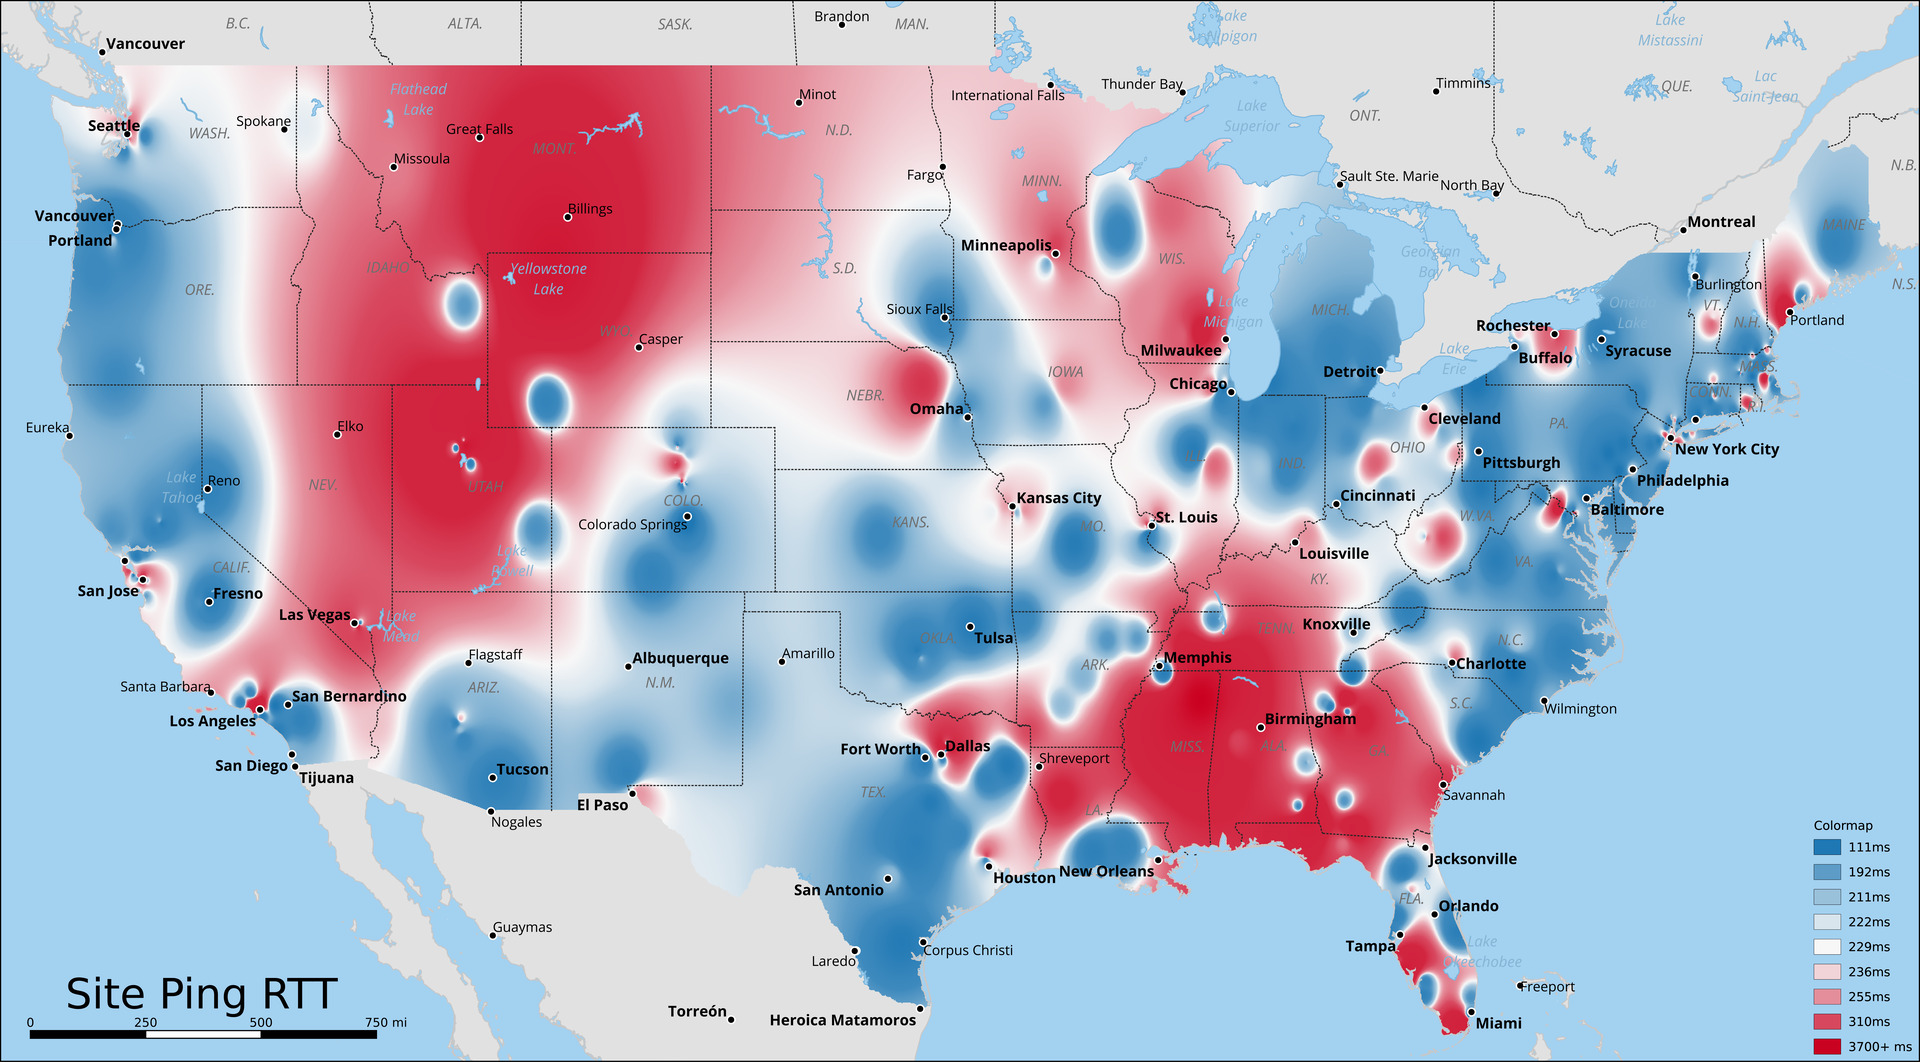
\includegraphics[width=0.85\textwidth]{images/siteping/site_ping_rtt_idw.jpg}
    \caption{Final Heat Map}
    \label{fig:siteping)_heatmap}
\end{figure}
